% XCircuit output "hbusstack.tex" for LaTeX input from hbusstack.ps
\def\putbox#1#2#3#4{\makebox[0in][l]{\makebox[#1][l]{}\raisebox{\baselineskip}[0in][0in]{\raisebox{#2}[0in][0in]{\scalebox{#3}{#4}}}}}
\def\rightbox#1{\makebox[0in][r]{#1}}
\def\centbox#1{\makebox[0in]{#1}}
\def\topbox#1{\raisebox{-0.60\baselineskip}[0in][0in]{#1}}
\def\midbox#1{\raisebox{-0.20\baselineskip}[0in][0in]{#1}}
\begin{center}
   \scalebox{0.8}{
   \normalsize
   \parbox{6.75in}{
   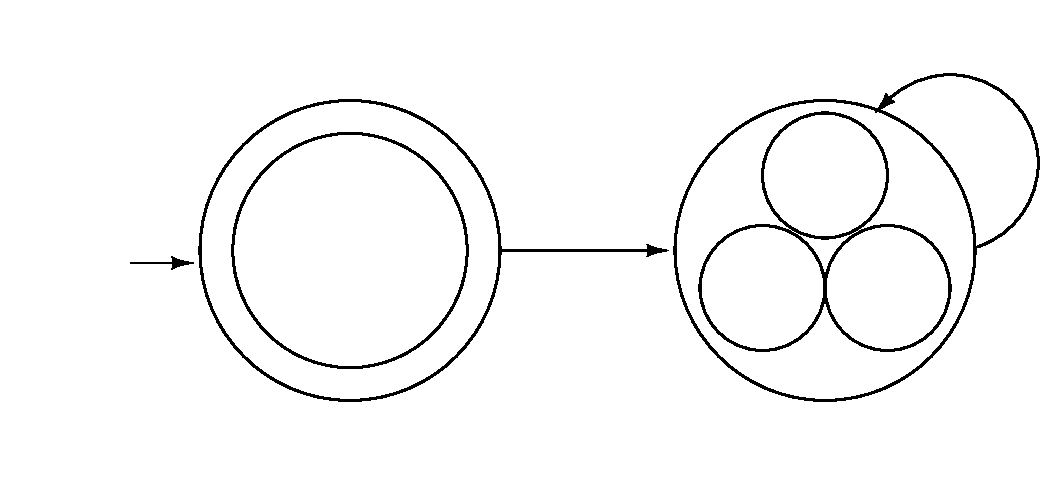
\includegraphics[scale=1]{hbusstack.ps}\\
   % translate x=1280 y=608 scale 0.38
   \putbox{4.31in}{2.97in}{1.20}{}%
   \putbox{1.72in}{1.47in}{1.20}{Inicialização}%
   \putbox{1.72in}{1.22in}{1.20}{Microcódigo}%
   \putbox{1.89in}{0.31in}{1.20}{}%
   \putbox{1.72in}{0.22in}{1.20}{Inicialização}%
   \putbox{1.97in}{0.06in}{1.20}{HBUS}%
   \putbox{4.81in}{0.22in}{1.20}{Ciclo HBUS}%
   \putbox{4.72in}{1.39in}{1.20}{Ciclo}%
   \putbox{4.72in}{1.14in}{1.20}{Micro}%
   \putbox{4.72in}{0.97in}{1.20}{código}%
   \putbox{4.81in}{1.22in}{1.20}{}%
   \putbox{5.56in}{1.39in}{1.20}{Ciclo}%
   \putbox{5.14in}{2.14in}{1.20}{Ciclo}%
   \putbox{5.47in}{1.14in}{1.20}{Inter-}%
   \putbox{5.47in}{0.97in}{1.20}{rupção}%
   \putbox{5.14in}{1.89in}{1.20}{Com.}%
   \putbox{5.14in}{1.72in}{1.20}{Serial}%
   \putbox{0.06in}{1.31in}{1.20}{RESET}%
   } % close 'parbox'
   } % close 'scalebox'
   \vspace{-\baselineskip} % this is not necessary, but looks better
\end{center}
